\documentclass[11pt]{article}

% Language setting
% Replace `english' with e.g. `spanish' to change the document language
\usepackage[english]{babel}

% Set page size and margins
% Replace `letterpaper' with `a4paper' for UK/EU standard size
\usepackage[letterpaper,top=2cm,bottom=2cm,left=3cm,right=3cm,marginparwidth=1.75cm]{geometry}

% Useful packages
\usepackage{amsmath}
\usepackage{graphicx}
\usepackage[colorlinks=true, allcolors=blue]{hyperref}
\usepackage{caption}
\usepackage{subcaption}
\usepackage{textcomp}
\usepackage{array}

% Title page package
%\usepackage{titling}

% Package for authors
%\usepackage{authblk}

% Setting font family
\renewcommand{\familydefault}{\rmdefault}

% Making commands for calculating word count 
\newcommand{\quickwordcount}[1]{%
\input{#1-words.sum}%
}
\newcommand{\thedate}{\today}

\begin{document}
%\linespread{1.5}
\begin{titlepage}
   \begin{center}
       \vspace*{2cm}

       \Huge
       \textbf{Mechanistic models out-perform phenomenological models in explaining bacterial population growth data}
            
       \vspace{2cm}

       \Large
       \textbf{Aditi Madkaikar} \\
       Word Count: \quickwordcount{main}

       \vfill
            
       MRes Computational Methods in Ecology and Evolution\\
            
       \vspace{0.6cm}
     
       Department of Life Sciences\\
       Imperial College London\\
       \thedate \\
            
   \end{center}
\end{titlepage} 

% Making the title page separate
\newpage

% Adding my abstract
\begin{abstract}
Bacterial population growth studies are used as a tool in many different fields like ecology, food science, and conservation. Obtaining a growth curve is challenging as most bacteria are unculturable in laboratory conditions and even after culturing there are many problems in quantifying and model fitting. In this project, I have tried to fit different linear and non-linear models to a bacterial population growth dataset to find out which model is the best fit for the data. The entire analysis was carried out in the form of a workflow. It can be reproduced by running the script run\_miniproject.sh. The analysis was carried out in R and the report used \LaTeX. The non-linear models used and mechanistic and have an overall better fit for the regular data subsets. At the same time, the phenomenological linear models show a better fit for the poor data subsets. Overall, the mechanistic models are a better fit for growth data than the phenomenological models. 
\end{abstract}

% Blankpage after abstract
\newpage

% Actual report
\section{Introduction}

Bacteria constitute the second-highest biomass on earth (after plants) \cite{doi:10.1073/pnas.1711842115} and play an important role as intermediates in the global carbon cycle balance. Bacteria are found in almost all habitats and play a big role in nutrient recycling. Bacterial population growth is studied [\cite{monod1949growth} in various branches of biology like physiology, genetics, ecology, food technology, and microbiology \cite{Kovarova-Kovar1998-hz}. In food science, bacterial population growth studies are used to estimate things like the time to food spoilage and the cause of food poisoning, which have clinical significance \cite{doi:10.1080/10408398.2011.570463}. In ecology, bacterial populations have been studied to understand their diversity and complexity in different environmental and metabolic conditions and the effect of changing environmental conditions on said populations, and their contributions to climate change. Other areas of study of microbial population growth include epidemiology, community ecology, and community assembly. Due to fast generation time, microbial populations can be used to test existing theories as well as build new ones. 

\begin{figure}[!ht]
\centering
    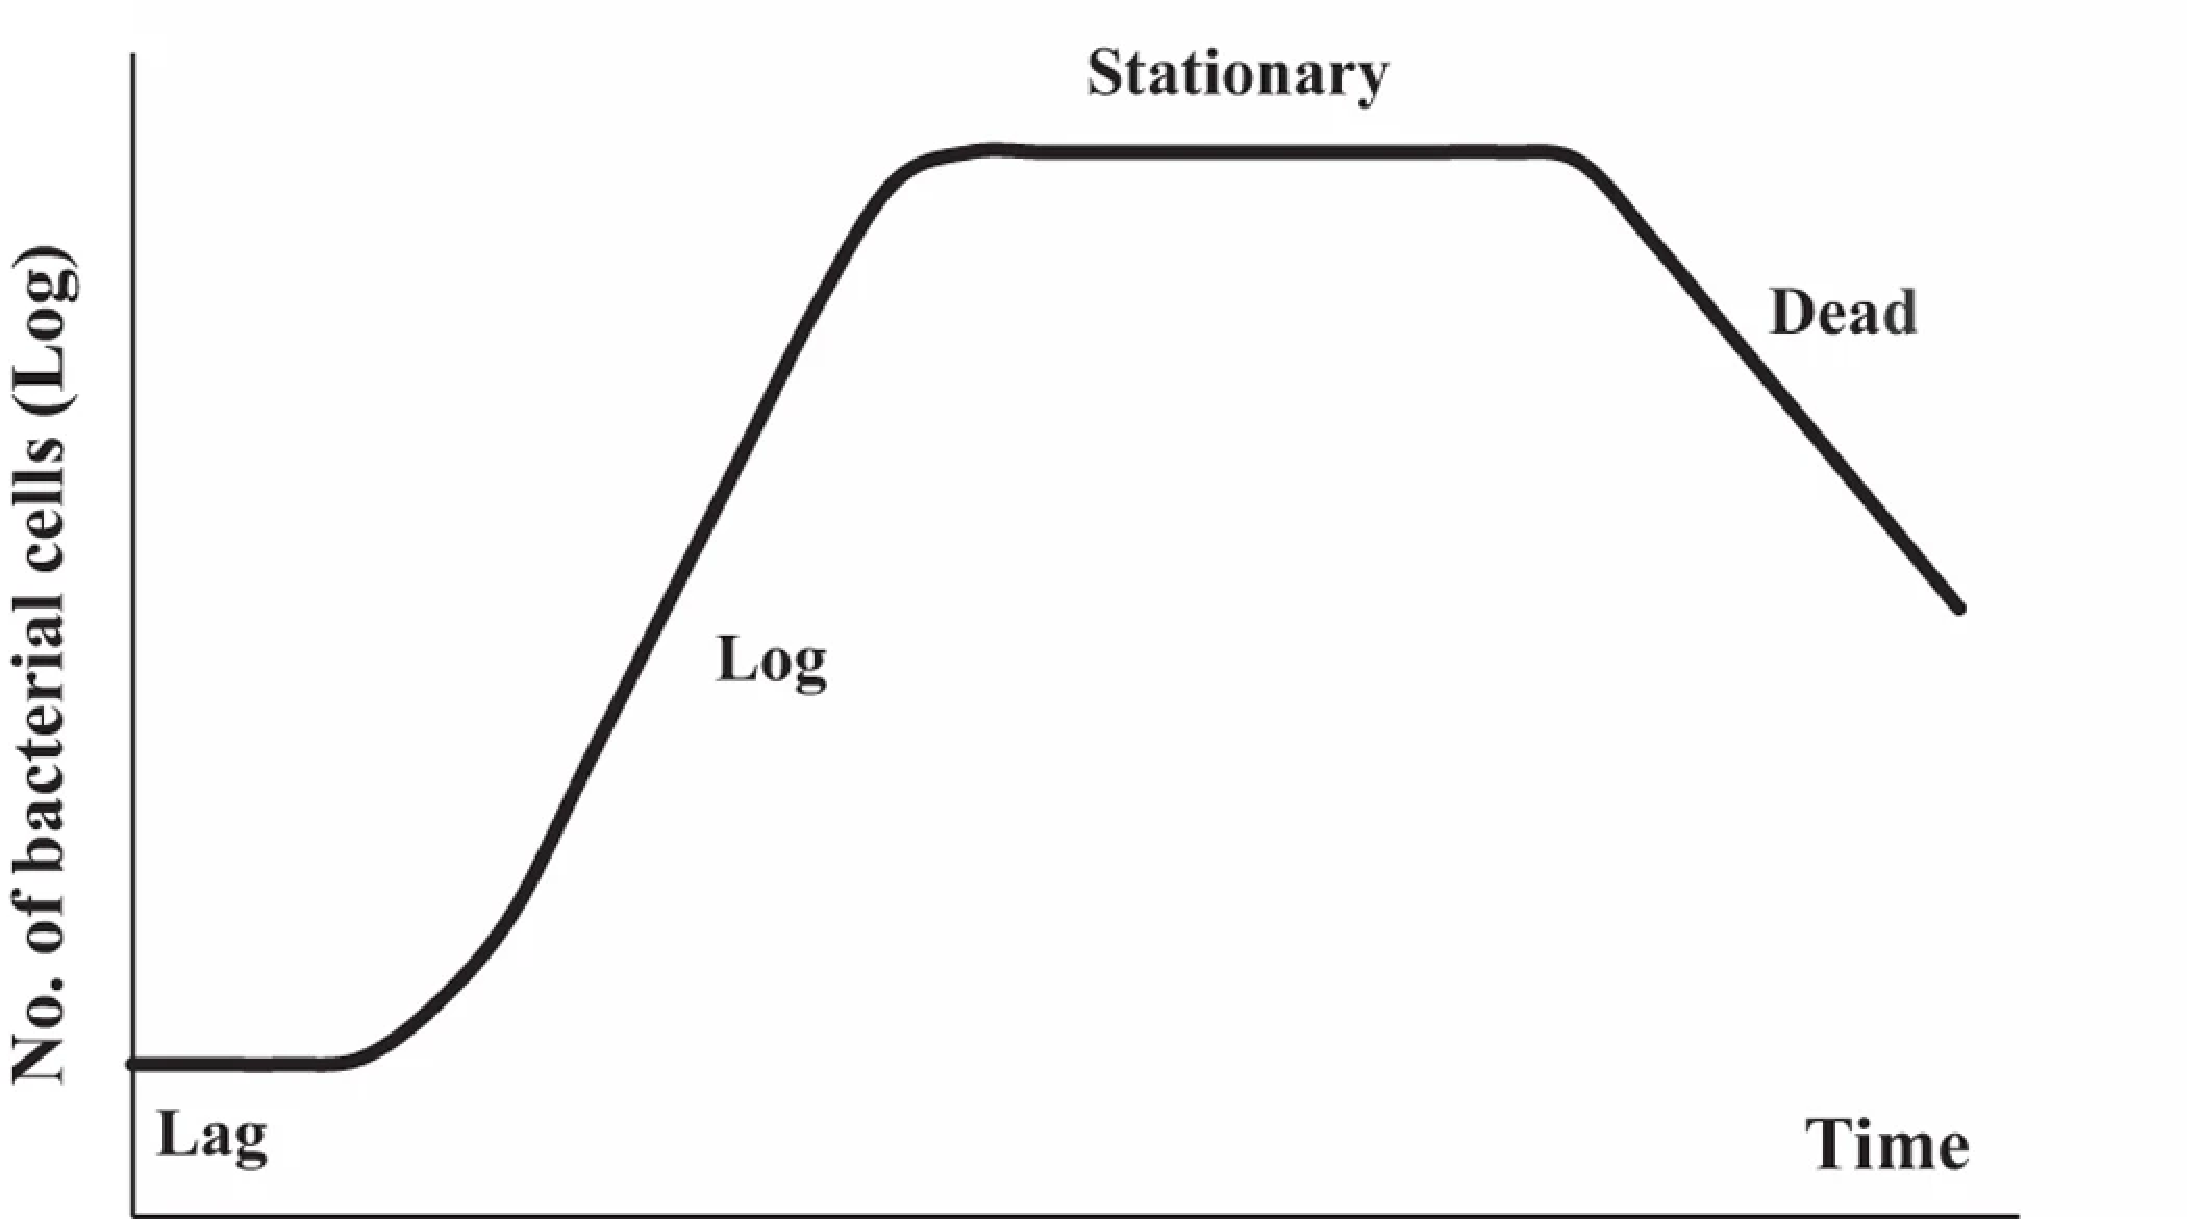
\includegraphics[width=.8\textwidth]{../data/curve.pdf}  
\caption{A typical bacterial population growth curve \cite{Wang2015-gf}}
\label{fig:figc}
\end{figure}

Characterization of bacterial population growth is difficult as most of the bacteria found in nature are unculturable \cite{doi:10.1128/JB.00345-12}. An added challenge is fitting models to bacterial culture data. In culture, the growth rate of bacteria goes through various phases \cite{monod1949growth} and is dependent on many parameters like temperature, pH, media composition, and the presence of toxins. Characterizing bacterial growth with so many complex parameters is very difficult and thus is generally done keeping the environmental and physiological parameters constant. Model fitting to bacterial population growth makes a few assumptions. The first is that population growth is exponential when there is no limit on resources and the abundance is low (cite Malthus). The second assumption is that the population goes through four stages: the 'lag phase', 'exponential phase', 'stationary phase', and 'death phase' \cite{doi:10.1080/10408398.2011.570463} \ref{fig:figc}. Over the years various mechanistic models like Logistic \cite{jason1983deterministic}, Gompertz, Stannard \cite{Zwietering1990-lp}, Baranyi, and Three-Phase Linear Models \cite{BUCHANAN1997313} have been built around these growth observations. These models take one or more of the different phases of bacterial growth curves into account. The question of whether to choose mechanistic models or phenomenological models to fit the data then arises. Phenomenological models make no assumptions about the data and thus can arguably fit better to a diverse dataset. On the other hand, mechanistic models are based on biological equations and thus can fit particular kinds of data better than their phenomenological counterparts. In this project, I compare the two types of models and their fits to bacterial growth data to identify which type fits the data better. Further, I also find the best-fitting model within phenomenological and mechanistic models. 

\section{Materials and Methods}

\subsection{Data Acquisition}

Population growth data for this analysis was obtained from the TheMulQuaBio. It contains data points from ten different experiments carried out under different environmental and physiological conditions. The experiments had a temperature range of 0-37\textdegree C and 18 different media. The population of bacteria was measured in four different units OD\_595 (Optical Density at 595nm), N (count number), CFU (Colony Formation Units), and Dry weight. For the purposes of this project, the population units have not been homogenized.  

\subsection{Computing Tools}

Analysis for this project was done using R(v4.1.2) \cite{R}. I made the decision to use R for the analysis because of the interactive interface available via RStudio \cite{RStudio}. In addition, R also provides easy ways for model fitting and data visualization. 

Apart from the functions available in base R, the following packages were used during the course of the project:
\begin{enumerate}
    \item tidyverse: This package contains tools useful for data manipulation and plotting. Loading this package also loads its dependencies (ggplot2, dplyr, tidyr, readr, etc). Most of the data wrangling and manipulation was done using tidyverse \cite{tidy}.
    \item minpack.lm: This package enables the use of the Levenberg-Marquardt algorithm to fit Non-linear models. The Non-linear models were fitted using this package \cite{minpack.lm}. This package was used as it does the model fitting using the Levenberg-Marquardt algorithm unlike the function available in base R.  
\end{enumerate}

The report is written in \LaTeX using \href{http://www.overleaf.com}{Overleaf} and compiled using a bash script written in the first week of the CMEE course. I used Overleaf as the editor for the report as it provides a good UI and lets the user visualize the rendered document. 

Python was not used in this workflow, but there are some steps that can be carried out with more ease using Python. 

Finally, the entire workflow and report compilation can be carried out using a single bash script (run\_miniproject.sh). The project has to be run in a Unix environment as the file paths for Unix and Windows are different.

\subsection{Data Analysis and Model fitting}
\subsubsection{Data Cleaning}
Firstly, I cleaned the data to remove negative values for Population and time. Then I created a unique ID by separating the experimental variables. The final version of this cleaned data was saved and used for further analyses.
\subsubsection{Linear Model Fitting}
The data was subsetted using the unique IDs (henceforth the original data will be referred to as the dataset and the subsetted data will be referred to as data subset(s)). The following three different linear models were fit to all data subsets to find the best-fitting model:

\begin{enumerate}
    \item \textbf{Linear Model of degree 1 (Straight line fit):} It is a phenomenological model of degree 1 (henceforth referred to as linear regression). 
    \begin{equation}
        log N_{t} = at + b
    \end{equation}
    \item \textbf{Quadratic Model:} It is a phenomenological model of degree 2.
    \begin{equation}
        log N_{t} = at^{2} + bt + c
    \end{equation}
    \item \textbf{Cubic Model:} It is a phenomenological model of degree 3.
    \begin{equation}
        log N_{t} = at^{3} + bt^{2} + ct + d
    \end{equation}
\end{enumerate}

In all the linear models, $log N_{t}$ is the population at time $t$ and $a, b, c, d$ are model paramters. 
\subsubsection{Non-linear Model fitting}
Again the data was subsetted based on the unique ID. The following non-linear models were fitted all data subsets which have more data points than the number of parameters in the model:
\begin{enumerate}
    \item \textbf{Logistic Model:} It is a phenomenological model which assumes that  it follows a sigmoidal curve \cite{jason1983deterministic}. This model was designed for data in normal scale. 
    \begin{equation}
    \begin{split}
        N_{t} = \frac{N_{0}Ke^{rt}}{K+N_{0}(e^{rt}-1)},
        \\
        log N_{t} = \frac{log N_{t} + log K + rt}{log ({K + N_{0}(e^{rt}-1)})}
    \end{split}
    \label{Logi}
    \end{equation}
    \item \textbf{Gompertz Model:} It is a mechanistic model that assumes the growth of microbial population follows an exponential curve after an initial time lag. This model was designed for log-transformed data \cite{Zwietering1990-lp}.
    \begin{equation}
        log N_{t} = N_0 + (K - N_{0})e^{-e^{r_{max}exp^{1}\frac{t_{lag}-t}{(K-N_{0})log 10}-1}}
    \label{Gompy}
    \end{equation}
\end{enumerate}

For the non-linear models, $N_{t}$ and $log N_{t}$ were the population and log of the population at time $t$. $K, r_max, N_{0}, t_{lag}$ are the carrying capacity, maximum growth rate, initial population, and time lag respectively. 

\subsection{Model Comparison}
All the models were fitted to the maximum possible data subsets. The model comparison could be done using the Akaike Information Criterion (AIC) which is an estimate of information lost during model fitting. To compare the different model fits, Small sample unbiased Akaike Information Criterion (AIC\textsubscript{c}) \cite{JOHNSON2004101} was used as few data subsets have very low sample sizes. AIC\textsubscript{c} was calculated using the following formula: 
\begin{equation}
    AIC_{c} = n + 2 + n log (\frac{2\pi}{n}) + n log RSS + 2p\frac{n}{n-p-1}
\label{AIC}
\end{equation}

Here, $RSS, n, p$ are the Residual sum of squares, sample size, and the number of model parameters respectively. 

\section{Results}

The dataset was split into 285 unique data subsets based on experimental and environmental parameters. 18 data subsets had 5 data points or fewer and thus all models couldn't be fitted to them. The Gompertz model was able to fit 261 data subsets and the linear regression was able to fit all data subsets \ref{tab:my_label}.

\begin{figure}[!ht]
\begin{subfigure}{.45\textwidth}
  \centering
  % include first image
  \includegraphics[width=.9\linewidth]{../results/pie_chart_lin.pdf}
  \caption{Best fitted model distribution (Linear models)}
  \label{fig1:sub-first}
\end{subfigure}
\begin{subfigure}{.45\textwidth}
  \centering
  % include second image
  \includegraphics[width=.9\linewidth]{../results/pie_chart_non_lin.pdf}  
  \caption{Best fitted model distribution (Non-linear models)}
  \label{fig1:sub-second}
\end{subfigure}
\caption{Best fitted model distribution}
\label{fig:fig1}
\end{figure}

\subsection{Linear Models}
The three linear models were fit to semi-log transformed data subsets. The linear regression had the highest mean AIC\textsubscript{c} values whereas the cubic model had the lowest. At the same time, the cubic model had four parameters and hence could be fitted to 267 data subsets whereas the linear regression could be fitted to all data subsets due to the low number of parameters. The quadratic model was able to fit more data subsets than the cubic model but also had higher AIC\textsubscript{c} \ref{fig2:sub-second}. In comparison, the cubic model was the best-fitting linear model \ref{fig1:sub-first}. 

\subsection{Non-Linear Models}
The two non-linear models were fitted to semi-log transformed data subsets. The Gompertz model could be fitted to 261 data subsets whereas the logistic model could be fitted to 277 data subsets. The Gompertz model had lower AIC\textsubscript{c} values than the logistic model \ref{fig2:sub-second}. In comparison, the Gompertz model had a better performance than the logistic model \ref{fig1:sub-second}. The advantage of the logistic model was that it could fit more data subsets as it had lower number of parameters. 

\begin{figure}[!ht]
\begin{subfigure}{.49\textwidth}
  \centering
  % include first image
  \includegraphics[width=.9\linewidth]{../results/pie_chart.pdf}
  \caption{Best fitted model}
  \label{fig2:sub-first}
\end{subfigure}
\begin{subfigure}{.49\textwidth}
  \centering
  % include second image
  \includegraphics[width=.9\linewidth]{../results/violin.pdf}  
  \caption{Violin plot of the AIC\textsubscript{c} values of all the data}
  \label{fig2:sub-second}
\end{subfigure}
\caption{Model comparison}
\label{fig:fig2}
\end{figure}

\begin{table}[!ht]
    \centering
    \begin{tabular}{ | m{3cm} | m{2.3cm}| m{5cm} | m{3cm} |} 
        \hline
        Model name & Number of parameters & Type of model & Number of fitted data subsets \\ 
        \hline
        Linear Regression  & 2 & Phenomenological \& Linear & 285 \\ 
        \hline
        Quadratic & 3 & Phenomenological \& Linear & 277 \\
        \hline
        Cubic & 4 & Phenomenological \& Linear &267 \\
        \hline
        Logistic & 3 & Mechanistic \& Non-Linear &277 \\
        \hline
        Gompertz & 4 & Mechanistic \& Non-Linear &261 \\
        \hline
    \end{tabular}
    \caption{Model Description}
    \label{tab:my_label}
\end{table}

\subsection{Overall Model Comparison}
Overall the non-linear models performed and explained the data better than the linear models. The Gompertz model was the best fitting model for the most number of data subsets \ref{fig2:sub-first}. Together the Logistic and Gompertz models were the best-fitting models for more than 75\% of the data subsets. The cubic and quadratic models had a poor overall performance despite being the better performing linear models \ref{fig2:sub-first}. Despite being the worst performing linear model, linear regression was the overall best fit for around 15\% of the data subsets. 

Most data subsets having sufficient data points (>5 data points) were best explained by the mechanistic non-linear models \ref{fig3:sub-first}. Few data subsets were best explained by the phenomenological linear models despite having sufficient data points \ref{fig3:sub-second}. The models with a higher number of parameters showed a poorer fit for data subsets having a very low sample size. 

\begin{figure}[!ht]
\begin{subfigure}{.49\textwidth}
  \centering
  % include first image
  \includegraphics[width=.9\linewidth]{../results/good_fit.pdf}
  \caption{Best fit: Gompertz Model}
  \label{fig3:sub-first}
\end{subfigure}
\begin{subfigure}{.49\textwidth}
  \centering
  % include second image
  \includegraphics[width=.9\linewidth]{../results/bad_fit.pdf}  
  \caption{Best fit: Cubic Model}
  \label{fig3:sub-second}
\end{subfigure}
\caption{Different kind of data subsets}
\label{fig:fig3}
\end{figure}

The mean AIC\textsubscript{c} (of all data subsets) of the linear regression was the highest whereas that of the Gompertz model was the lowest \ref{fig2:sub-second}. The AIC\textsubscript{c} values of all the models were focused around the mean. The logistic model had the most widespread distribution of AIC\textsubscript{c} values and the Gompertz model had the least spread distribution. The linear regression and logistic model show extremely high AIC\textsubscript{c} values for a few data subsets. 

\section{Discussion}

Computationally, this project is done completely in R. It is possible to do a part or the entire project in another programming language like Python. Doing the project in multiple languages can optimize and make the workflow faster and more efficient. I used R due to a personal preference for the RStudio IDE. The main run script (run\_miniproject.sh) can also be written in Python. As it is a shell script it can only be run in a Unix environment as the file paths for Windows are different. Writing the script in Python can potentially make it usable even in the Windows environment. 

The aim of this project was to find which model best fits the given data and compare the different models used. The data used was the bacterial population growth dataset and the population growth with time was modeled. Apart from the temperature and species variation in the dataset, different culture media were used. Some of these media were growth media whereas others are food media (chicken breast, milk, beef). This could potentially lead to a bias in the data since most of the data was collected from food science-related studies investigating food spoilage, where bacterial growth may have been controlled.

Five models were fit to the data (three linear and two non-linear). All the models were built on the assumption that the data has no measurement errors in the explanatory variables, and the explanatory variables were not highly correlated. The linear models make no assumptions about the shape of the data and the coefficients have no biological meaning. All the linear models used were phenomenological deterministic models. The non-linear models used were mechanistic deterministic models and their coefficients carry biological meaning and are based on bacterial population growth assumptions. The logistic model was based on the sigmoid curve and calculated the population growth on a linear scale while the Gompertz model calculated population growth on the log scale. It assumed that the data has an initial stationary phase followed by an exponential growth phase and the stationary phase. It did not account for the death phase of the bacterial population. 

For comparing the models, all the residuals to be compared have to be on the same scale, I converted the logistic model to the log scale and carried out the fitting for linear models in the log scale for ease of AIC\textsubscript{c} calculation and model comparison. AIC\textsubscript{c} calculation can only be done when the residuals are normally distributed along the model fit. To check the distribution of residuals, I plotted explanatory plots. 

An alternate method to carry out model comparison would have been to convert all the residuals to the normal scale and then calculate AIC\textsubscript{c}.
I chose to convert my logistic model to log scale based on the classical equation of population growth. 

Overall, the non-linear models fit the data better than the linear models. This could be due to the models being mechanistic, the principles on which the models were built, and their relationship to ideal bacterial population growth \ref{fig3:sub-first}. Among the linear models, the cubic model was the best fitting\ref{fig1:sub-first}. A reason for this could be that the cubic curve has two inflection points and the slope of the growth also changes twice. Some of the data is poor data (very small sample size and/or not a sigmoidal shape) and it caused the non-linear models to give higher values of AIC\textsubscript{c}. In such cases, the linear models which do hot have any assumptions fit better than the non-linear models \ref{fig3:sub-second}.

The goal of this project was to find the model which fits the maximum data and not to find the model which best fits a given subset. In order to do so, the precision in model fitting was lost \cite{10.2307/27836590} to accommodate for generality. This project could only explain the general trend in microbial population growth and which model explains most of the data and not a specific trait. To carry out a more detailed study, the data has to be analyzed in smaller subsets with the goal of finding specific patterns. To expand this study, specific questions like the effect of temperature on microbial growth in a fixed media could be asked. 

\bibliographystyle{apalike}
\bibliography{ref}

\end{document}